\documentclass[a4paper,twoside]{ctexart}
\usepackage{geometry}
\geometry{margin=1cm,vmargin={0pt,1cm}}
\setlength{\topmargin}{-2cm}
\setlength{\paperheight}{23cm}
\setlength{\paperwidth}{18cm}
\setlength{\textheight}{19.6cm}
\setlength{\textwidth}{15cm}
\usepackage{makecell}
\usepackage{fancyhdr}
\usepackage{siunitx}
\usepackage{amssymb}
\usepackage{indentfirst}
\setlength{\parindent}{0.5em}

\pagenumbering{arabic}

% useful packages.
\usepackage{multirow}
\usepackage{caption}
\usepackage{mathrsfs}
\usepackage{amsfonts}
\usepackage{amsmath}
\usepackage{amsthm}
\usepackage{enumerate}
\usepackage{xcolor,graphicx,float,subfigure}
\usepackage{epstopdf}
\usepackage{multicol}
\usepackage{fancyhdr}
\usepackage{layout}
\usepackage{listings}
\lstset{language=Matlab}
\lstset{breaklines}
\lstset{extendedchars=false}
\usepackage[colorlinks,linkcolor=blue]{hyperref}
\usepackage{xcolor}
\usepackage{cite}
\usepackage[numbers,sort&compress]{natbib}
\setcitestyle{open={},close={}}
%\usepackage{natbibspacing}
%\renewcommand{\refname}{}
\usepackage{anyfontsize}

% 中文定理环境
\newtheorem{theorem}{定理}[section]
\newtheorem{lemma}[theorem]{引理}
\newtheorem{proposition}[theorem]{命题}
\newtheorem{corollary}[theorem]{推论}
\newtheorem{definition}{定义}[section]
\newtheorem{example}{例}[section]
\newtheorem{remark}{注}[section]
\newenvironment{solution}{\begin{proof}[\indent\bf 解]}{\end{proof}}
\renewcommand{\proofname}{\bf 证明}

% % English theorem environment
% \newtheorem{theorem}{Theorem}[section]
% \newtheorem{lemma}[theorem]{Lemma}
% \newtheorem{proposition}[theorem]{Proposition}
% \newtheorem{corollary}[theorem]{Corollary}
% \newtheorem{definition}{Definition}[section]
% \newtheorem{remark}{Remark}[section]
% \newtheorem{example}{Example}[section]
% \newenvironment{solution}{\begin{proof}[Solution]}{\end{proof}}

% some common command
\newcommand{\dif}{\mathrm{d}}
\newcommand{\avg}[1]{\left\langle #1 \right\rangle}
\newcommand{\pdfrac}[2]{\frac{\partial #1}{\partial #2}}
\newcommand{\op}{\odot}
\newcommand{\Eabs}{E_{\mathrm{abs}}}
\newcommand{\Erel}{E_{\mathrm{rel}}}
\newcommand{\Ediv}{\mathrm{div}}%\div是除号
\newcommand{\lrq}[1]{\left( #1 \right)}
\newcommand{\avint}[1]{\frac{1}{\left|#1\right|}\int_{#1}}

\newcommand{\upcite}[1]{\textsuperscript{\textsuperscript{\cite{#1}}}} 

\makeatletter
\newcommand\sixteen{\@setfontsize\sixteen{17pt}{6}}
\renewcommand{\maketitle}{\bgroup\setlength{\parindent}{0pt}
\begin{flushleft}
\sixteen\bfseries \@title
\medskip
\end{flushleft}
\textit{\@author}
\egroup}
\renewcommand{\maketag@@@}[1]{\hbox{\m@th\normalsize\normalfont#1}}
\makeatother

\CTEXsetup[format={\Large\bfseries}]{section}

\title{Surface Diffusion 数学文档}


\begin{document}
\maketitle


\section{方程描述}
表面扩散流是一个四阶方程,其在二维情形下对闭曲线的作用和在三维情
形下对闭曲面的作用可以用以下演化方程描述:
\begin{eqnarray}
  \begin{aligned}
  v_n = \begin{cases}
 \partial_{ss}{\kappa} \quad \text{in 2D},\\
 \Delta_s\mathcal{H}   \quad \text{in 3D},
\end{cases}
  \label{eq:geneequ}
  \end{aligned}
\end{eqnarray}
这里$v_n$是沿外法向的速度,$\kappa$表示二维曲线的曲率,$s$是弧长参数;
$\mathcal{H}$表示三维曲面的平均曲率,$\Delta_s$表示曲面上的
Laplace–Beltrami算子,即$\Delta_s := \nabla_s\cdot \nabla_s$,这里
$\nabla_s$表示曲面上的梯度算子。表面扩散流有两个最基本的几何性质:

(1)二维情形下,曲线所围的面积保持不变;三维情形下,曲面包围的体积保持
不变。

(2)二维情形下,曲线的总弧长随时间递减;三维情形下,曲面的总表面积递减。


我们的研究对象是二维表面扩散流,我们将其定义如下:
\begin{definition}[二维表面扩散流问题]
    \label{eq:defequ}
对于嵌入二维平面$\mathbb{R}$中的随时间变化的简单闭合曲线
$\boldsymbol X:[0,L(t)]\times[0,+\infty) \rightarrow
\mathbb{R}^2$,二维表面扩散流方程满足
\begin{eqnarray}
  \begin{aligned}
  \pdfrac{\boldsymbol X}{t} = \frac{\partial^2\kappa}{\partial s^2}\boldsymbol n, s\in[0,L(t)],
  t\in[0,+\infty),\\
  \boldsymbol X(s,0) = \boldsymbol X_0(s), s\in[0,L_0].
  \label{eq:oriequ}
  \end{aligned}
\end{eqnarray}
其中$s$表示弧长,$\kappa$表示曲线对应点处的曲率,$L(t)$为曲线在$t$时刻
的总弧长,$\boldsymbol n$为曲线对应点处的单位外法向量。二维表面扩散流问题
即是在给定初始简单闭合曲线$\boldsymbol X(s,0)$的情况下,求解二维表面扩散
流方程在任意$t \ge 0$时刻的解。
\end{definition}

为了空间离散和误差分析的方便,我们重写\eqref{eq:oriequ}的右端项。注意
到
\begin{equation}
  \kappa = -\frac{\partial^2\boldsymbol X}{\partial s^2}\cdot \boldsymbol n,
  \label{eq:curv}
\end{equation}
以及$\boldsymbol n$在二维情形下具有形式
\begin{equation}
  \label{eq:onor}
  \boldsymbol n = (\pdfrac{\boldsymbol X_y}{s},-\pdfrac{\boldsymbol X_x}{s})^{\text{T}}.
\end{equation}
因此,\eqref{eq:curv}可以改写为
\begin{equation}
  \label{eq:rcurv}
  \kappa = -\frac{\partial^2\boldsymbol X_x}{\partial
    s^2}\pdfrac{\boldsymbol X_y}{s} + \frac{\partial^2\boldsymbol X_y}{\partial
    s^2}\pdfrac{\boldsymbol X_x}{s}.
\end{equation}
这里$\boldsymbol X_x,\boldsymbol X_y$分别是$\boldsymbol X$在$x$和$y$方向上的分
量。
\section{表面扩散流性质描述}
\subsection{解的存在性与唯一性}
二维表面扩散流解的存在性研究的主要工作由Elliott 和 Garcke 完成\textsuperscript{\cite{ref1}},他们证
明了在$C^4$初值条件下解的局部存在性和正则性,并且在解的整体存在性的假
设下证明了任何闭曲线在表面扩散流的作用下将趋于正圆。下面几个定理给出了
完整的说明。
\begin{theorem}[解的局部存在性]
  假设$\boldsymbol X_0\in C^4(I)\cap \mathcal{M}_{\delta_0/2}$,其中$I$是
  $\mathbb{R}$上的紧集,$\boldsymbol X_0:I\rightarrow \mathcal{M}^0$,$\mathcal{M}_{\delta}$定义为
  \begin{equation}
    \label{eq:mathcalM}
    \mathcal{M}_{\delta} := \{\ d \in C^1(I)\ |\ \left \|d  \right
    \|_{C^1(I)}<\delta ,  d \text{是周期函数}\}.
  \end{equation}
  则$\forall \epsilon \in (0,1],$有\\
  $(a)$ 存在一个时刻$T>0($依赖$\epsilon)$,使得方程\eqref{eq:oriequ}
  存在一个解
  \begin{equation}
    \boldsymbol X \in L^{\infty}(0,T;H^2(I))\cap L^{2}(0,T;H^4(I))\cap
    H^{1,2}(0,T;L^2(I))\cap C^{0}([0,T];\mathcal{M}_{\delta_0})
    \label{eq:exist}
  \end{equation}
  满足$\boldsymbol X(0) = \boldsymbol X_0$。\\
  $(b)$ 存在一个$\delta_1>0$,$\delta_1$依赖于$\mathcal{M}^0($但与
  $\epsilon$无关$)$,使得方程\eqref{eq:oriequ}存在一个具有$(a)$中正则性
  的解$\boldsymbol X$,只要
  $$\sup_{0\le t\le T}\left \|\boldsymbol X(t) - \boldsymbol X(0)  \right
  \|_{C^1(I)} < \delta_1,$$
  则$\boldsymbol X$可以被延拓。
\end{theorem}
\begin{theorem}[近圆初值条件下解的整体存在性]
  对任意半径$R_0>0$,存在$\delta(R_0)>0$,使得对所有初值条件
  $\boldsymbol X_0$,只要$\boldsymbol X_0$满足\\
  $(a)$ $\boldsymbol X_0$具有形式$\boldsymbol X_0 =
  \{d_0(\theta)(\cos{\theta},\sin{\theta})^T|\theta \in [0,2\pi)
   \text{且} d_0\text{是周期函数} \},$\\
  $(b)$ $\int_{\boldsymbol X_0}\kappa_0^2 $是有界的,\\
  $(c)$ $\left \|d_0 - R_0  \right \|_{C^1([0,2\pi))}\le \delta(R_0)
  ,$\\
  $(d)$ $\int_{\boldsymbol X_0}\kappa_s(0)^2 \le  \delta(R_0)$,\\
  则方程\eqref{eq:oriequ}具有整体解。
\end{theorem}
\begin{theorem}[整体解存在的假设下表面扩散流的作用]
假设方程\eqref{eq:oriequ}存在单连通的整体解,则存在一个时刻$T_0$,使得
对任意$t > T_0$,$\boldsymbol X_t$具有以下形式:
$$\boldsymbol X_t = \{(x_0(t),y_0(t))^T +
R(\theta,t)(\cos{\theta},\sin{\theta})^T|\theta \in [0,2\pi) \},$$
其中$R(\cdot,t):[0,2\pi) \rightarrow \mathbb{R}^+$是周期函数。进一步,
有\\
$(a)$ $L(t) \searrow L_{\infty},$ 以及\\
$(b)$ $\left \| R(\cdot,t) - R_{\infty} \right \| \longrightarrow 0 $,\\
这里$L(t)$表示$t$时刻曲线的总弧长,$L_{\infty}$和$R_{\infty}$分别表示面积与
$\boldsymbol X_0$所围区域面积相同的圆的弧长与半径。
\end{theorem}
以上三个定理给出了方程\eqref{eq:oriequ}解的存在性,但没有得到唯一性的
结果。唯一性的工作由 Polden 和 Giga、Ito 各自独立完成\textsuperscript{\cite{ref2},\cite{ref3}},他们都对$H^4$初
值曲线证明了局部解的唯一性。Escher, Simonett 和 Mayer 把工作推
广到任意维度上的超表面,对$h^{2+\beta}(0<\beta<1)$的初值条件给出了局
部解的存在性、光滑性和唯一性\textsuperscript{\cite{ref4}}。其最主要的结果如下。\\
\indent 首先对相关记号加以说明。设$U\in \mathbb{R}^n$是开集,令$h^s(U)$表示 order 为$s$ 的 little
Hölder 空间,即 $BUC^{\infty}(U)$在$BUC^{s}(U)$中的闭包,这里
$BUC^{s}(U)$表示$U$上所有有界、$s$阶一致 Hölder 连续的函数构成的 Banach 空
间。
\begin{theorem}[$h^{2+\beta}$初值条件下解的存在性、光滑性和唯一性]
  \label{thm:exist}
假设$0<\beta<1$,$\boldsymbol X_0$是$\mathbb{R}^n$中一个紧、闭、浸入$\left(immersed \right)$
的超曲面,且$\boldsymbol X_0 \in h^{2+\beta}$,则存在某个$T > 0$,表面扩散流方程存在唯一的局部解$\boldsymbol X =
\{ \boldsymbol X(t);t\in[0,T)\}$。在$[0,T)$上,$\boldsymbol X(t) \in
C^{\infty}$。进一步,在$[0,T)$上,映射$[t \mapsto \boldsymbol X(t)]$在
$h^{2+\beta}$拓扑下是连续的,在$C^{\infty}$拓扑下是光滑的。\\
  \end{theorem}
这些工作为我们数值求解表面扩散方程
奠定了理论基础。
\subsection{面积保持与弧长收缩}
二维表面扩散流有两个基本的几何性质,即面积保持和弧长收缩。
\begin{theorem}[面积保持与弧长收缩]若$\boldsymbol X(t)$是表面扩散流
  \eqref{eq:oriequ}的解,令$A(t)$表示
约当曲线$\boldsymbol X(t)$围成区域的有向面积,$L(t)$表示$\boldsymbol X(t)$的总弧
长。则
\begin{eqnarray}
  \label{eq:essgeo}
  \frac{\mathrm{d}}{\mathrm{d} t} A(t) =
  \int_{\boldsymbol X(t)}(\pdfrac{\boldsymbol X}{t} \cdot
  \boldsymbol n)\text{d} s =
  \int_{\boldsymbol X(t)}\frac{\partial^2\kappa}{\partial s^2} \text{d} s \equiv
  0, \quad t \ge 0 ,\\
  \frac{\mathrm{d}}{\mathrm{d} t} L(t) =
  \int_{\boldsymbol X(t)}(\pdfrac{\boldsymbol X}{t} \cdot \boldsymbol n)\kappa
  \text{d} s = -\int_{\boldsymbol X(t)}\left |\pdfrac{\kappa}{s}  \right
  |^2 \text{d} s
  \le 0, \quad t \ge 0.
\end{eqnarray}
即在表面扩散流的作用下,随着时间的推移,曲线的有向面积不变而弧长不增。
\end{theorem}

\subsection{表面扩散流的其它性质}
考虑到后续的理论分析需要,这里列出表面扩散流的几条性质\textsuperscript{\cite{ref5}}。这些性质多数与
曲率流有所不同,在设计离散格式时要给予相应的关注。
\begin{itemize}
\item (不保凸性) 存在充分光滑的凸约当曲线,当以该曲线作为方程
  \eqref{eq:oriequ}的初值时,在唯一解的存在区间内,解不再具有凸性。
\item (不保嵌入性$\left(embeded\right)$) 存在充分光滑的嵌入约当曲线,当以该曲线作为方程
  \eqref{eq:oriequ}的初值时,在奇点产生前,曲线不再具有嵌入性。这也会
  导致解的光滑性的丢失。
\item (无极值原理) \eqref{eq:oriequ} 是一个非线性四阶抛物方程,它不满
  足极值原理,而极值原理是二阶抛物方程最重要的性质之一。作为直接推论,
  无碰撞原则不再成立,即无法保证初始无交点的两条约当曲线在表面扩散流作
  用下不相交,可能的拓扑结构变化会带来计算和分析的困难。
\end{itemize}
\section{离散格式设计}
为了实现与现有二维MARS界面追踪方法的耦合,我们有两个基本任务:其一是通
过空间离散给出任一时刻方程\eqref{eq:oriequ}右端项的近似值,即这一时刻
曲线上示踪点的速度场;其二是在给定速度场的前提下,选用合适的时间积分方法
完成界面追踪过程。
\subsection{空间离散格式}
\label{sec:discrete}
空间离散的主要任务是:对边界样条曲线上的一列示踪点列,通过空间离散,在
二阶/四阶精度的要求下给出每个示踪点处的流速场$\boldsymbol V_i := \pdfrac{\boldsymbol X_i}{t}$,从而实现
与二维MARS方法的耦合。\\
\indent 我们选用有限差分方法对方程\eqref{eq:oriequ}的右端项进行离散。首先对弧
长进行估计。设边界样条曲线上示踪点列序列为$\bar{\boldsymbol X} =
\left(\bar{\boldsymbol X}_1,\bar{\boldsymbol X}_2,\cdots,\bar{\boldsymbol X}_{N+1}\right)$
,其中$\bar{\boldsymbol X}_1 = \bar{\boldsymbol X}_{N+1}$。则样条曲线上从
$\bar{\boldsymbol X}_i$到$\bar{\boldsymbol X}_{i+1}$的弧长为
\begin{equation}
  \label{eq:calarclen}
  s_i = \int_{l_i}^{l_{i+1}}\sqrt{S_x'(l)^2 + S_y'(l)^2}\text{d}l, 
\end{equation}
其中$S_x(l),S_y(l)$为以$l$为拟合参数的样条曲线函数,即$l$是样条曲线的
累计弦长。$\bar{\boldsymbol X}_i$处的对应参数为$l_i$。为了让表面扩散流计
算达到二阶/四阶精度,我们采用三点/四点Gauss-Legendre公式计算\eqref{eq:calarclen},
这一公式有五阶/七阶的代数精度。通过计算得到近似弧长$\bar{s}_i$。\\
\indent 在得到上述近似弧长的基础上,我们用差分格式近似计算空间导数$\frac{\partial^2\boldsymbol X_i}{\partial
    s^2},\pdfrac{\boldsymbol X_i}{s}$,从而根据\eqref{eq:onor},
  \eqref{eq:rcurv}得到近似的外法向$\bar{\boldsymbol n}_i$和近似曲率
  $\bar{\kappa}_i$。为了达到二阶精度,这里分别对一阶和二阶导数采用五点和六点格式,即四阶差分方法。
  \begin{eqnarray}    
    \pdfrac{\bar{\boldsymbol X}_i}{s} =
    \boldsymbol f_{\bar{s},4}^{(1)}(\bar{\boldsymbol X}_i,t) =
    \sum_{j=i-2}^{i+2}\alpha_{\bar{s},4,i,j}^{(1)}(\bar{\boldsymbol X},t)
    \bar{\boldsymbol X}_j,
    \label{eq:calder1}\\
    \frac{\partial^2\bar{\boldsymbol X}_i}{\partial s^2} =
    \boldsymbol f_{\bar{s},4}^{(2)}(\bar{\boldsymbol X}_i,t) =
    \sum_{j=i-2}^{i+3}\alpha_{\bar{s},4,i,j}^{(2)}(\bar{\boldsymbol X},t)
    \bar{\boldsymbol X}_j,
    \label{eq:calder2}
  \end{eqnarray}
  这里$\boldsymbol f$和$\alpha$的下标$\bar{s}$表示关于近似弧长$\bar{s}_i$
  的离散,上标$(k)$表示对$k$阶导数的离散,下标$4$表示四
  阶。离散格式的具体系数$\alpha_{\bar{s},4,i,j}^{(k)}(\bar{\boldsymbol X},t)$可以通过拉格朗日插
  值求$k$阶导数得到:
  
  \begin{footnotesize}
    \begin{eqnarray}
    \begin{aligned}
      \label{eq:dercoe1}      
  \alpha_{\bar{s},4,i,i-2}^{(1)} & =
  \frac{\bar{s}_{i-1}\bar{s}_{i}(\bar{s}_{i}+\bar{s}_{i+1})}{\bar{s}_{i-2}(\bar{s}_{i-2}+\bar{s}_{i-1})(\bar{s}_{i-2}+\bar{s}_{i-1}+\bar{s}_{i})(\bar{s}_{i-2}+\bar{s}_{i-1}+\bar{s}_{i}+\bar{s}_{i+1})},
  \\
  \alpha_{\bar{s},4,i,i-1}^{(1)} &= \cdots\\
  \vdots\\
  \alpha_{\bar{s},4,i,i+2}^{(1)} &= \cdots
\end{aligned}
  \end{eqnarray}
\begin{eqnarray}
\begin{aligned}
      \label{eq:dercoe2}
  \alpha_{\bar{s},4,i,i-2}^{(2)} &=
  \frac{-2(3\bar{s}_{i}^2\bar{s}_{i-1}\! -\!2\bar{s}_{i}^2\bar{s}_{i+1}\! -\!\bar{s}_{i}^2\bar{s}_{i+2}\! -\!\bar{s}_{i}\bar{s}_{i+1}^2\! +\!\bar{s}_{i+1}^2\bar{s}_{i-1}\! -\!\bar{s}_{i}^3\! -\!\bar{s}_{i}\bar{s}_{i+1}\bar{s}_{i+2}\! +\!4\bar{s}_{i}\bar{s}_{i+1}\bar{s}_{i-1}\! +\!2\bar{s}_{i}\bar{s}_{i+2}\bar{s}_{i-1}\! +\!\bar{s}_{i+1}\bar{s}_{i+2}\bar{s}_{i-1})}{\bar{s}_{i-2}(\bar{s}_{i-2}+\bar{s}_{i-1})(\bar{s}_{i-2}+\bar{s}_{i-1}+\bar{s}_{i})(\bar{s}_{i-2}+\bar{s}_{i-1}+\bar{s}_{i}+\bar{s}_{i+1})(\bar{s}_{i-2}+\bar{s}_{i-1}+\bar{s}_{i}+\bar{s}_{i+1}+\bar{s}_{i+2})},
  \\
  \alpha_{\bar{s},4,i,i-1}^{(2)} &= \cdots\\
  \vdots\\
  \alpha_{\bar{s},4,i,i+3}^{(2)} &= \cdots
  \end{aligned}                               
\end{eqnarray}
\end{footnotesize}
\indent 如果需要四阶精度,只需要将五点/六点格式替换为七点/八点格式,即使用六阶精度的空间离散。\\
\indent 通过\eqref{eq:onor},
  \eqref{eq:rcurv}得到近似的外法向$\bar{\boldsymbol n}_i$和近似曲率
  $\bar{\kappa}_i$后,我们用一样的方式计算
  $\frac{\partial^2\kappa}{\partial s^2}$:
  \begin{equation}
    \label{eq:calderkappa}
    \frac{\partial^2\bar{\kappa}_i}{\partial s^2} =
    \boldsymbol f_{\bar{s},4}^{(2)}(\bar{\kappa}_i,t) = \sum_{j=i-2}^{i+3}\alpha_{\bar{s},4,i,j}^{(2)}(\bar{\kappa},t) \bar{\kappa}_j,
  \end{equation}
  式中的$\alpha_{\bar{s},4,i,j}^{(2)}(\bar{\kappa},t)$与
  \eqref{eq:dercoe2}相同。最后,我们通过
  \begin{equation}
    \label{eq:calv}
    \bar{\boldsymbol V}_i = \frac{\partial^2\bar{\kappa}_i}{\partial s^2}
    \bar{\boldsymbol n}_i
  \end{equation}
  得到流速场的近似。至此,完整的空间离散格式说明完毕。
  \subsection{时间积分方法}
  \label{sec:timeintegral}
  在完成空间离散后,我们可以将方程$\pdfrac{\bar{\boldsymbol X_i}}{t} =
  \bar{\boldsymbol V}_i$及其初值条件写成如下统一的常微分方程组形式,从而
  得到初值问题:
  \begin{eqnarray}
  \begin{aligned}
  \pdfrac{\bar{\boldsymbol X}}{t} &=
  \boldsymbol f_{\bar{s}}(\bar{\boldsymbol X},t),\quad t\in[0,+\infty),\\
  \bar{\boldsymbol X}(0) &= \bar{\boldsymbol X}^0.
  \label{eq:nODEs}
  \end{aligned}
  \end{eqnarray}
  设$t_n$时刻示踪点列为$\bar{\boldsymbol X}^n$,时间步长为$k$,即
  $t_{n+1} = t_n + k$,则需要通过以下时间积分来得到$t_{n+1}$时刻的示踪
  点位置:
  \begin{equation}
    \label{eq:exintegral}
    \bar{\boldsymbol X}^{n+1} = \bar{\boldsymbol X}^n + \int_{t_n}^{t_{n+1}}\boldsymbol f_{\bar{s}}(\bar{\boldsymbol X},t)\text{d}t.
  \end{equation}
  值得注意的是,由于方程是自治(autonomous)的,即右端项不显式地依赖于
  $t$,因此下面我们把$\boldsymbol f_{\bar{s}}(\bar{\boldsymbol X},t)$
  简写为$\boldsymbol f_{\bar{s}}(\bar{\boldsymbol X})$。\\
  \indent 由于方程\eqref{eq:nODEs}的右端项的雅可比矩阵(具体计算见
  \ref{calJacobi}节)会有绝对值很大的负特征值,即问题是刚性的,出于稳定
  性的考虑,我们选用对角隐式 Runge-Kutta 方法 (DIRK) 来进行初值问题的求解。
  DIRK 方法是系数矩阵 $A$ 为下三角矩阵的隐式 Runge-Kutta 方法,具体形
  式如下:
  \begin{equation}
    \label{eq:DIRK}
  \left\{
\begin{aligned}
 &\boldsymbol Z_1= \bar{\boldsymbol X}^n + ka_{1,1} \boldsymbol f_{\bar{s}}(\boldsymbol Z_1), \\
 &\boldsymbol Z_i= \bar{\boldsymbol X}^n + k{\textstyle \sum_{j=1}^{i-1}}a_{i,j}
 \boldsymbol f_{\bar{s}}(\boldsymbol
 Z_j)+ka_{i,i}\boldsymbol f_{\bar{s}}(\boldsymbol Z_i),i =
 2,\cdots,\text{nstage},\\
 &\bar{\boldsymbol X}^{n+1} = \bar{\boldsymbol X}^n + k{\textstyle
   \sum_{j=1}^{\text{nstage}}}b_j\boldsymbol f_{\bar{s}}(\boldsymbol Z_j),
\end{aligned}
\right.
\end{equation}
其中 $k$ 为时间步长,nstages 为 DIRK 方法的步数,$a$ 和 $b$ 为 DIRK 方法 Butcher 表中的系
数。其中的每一步可以如下牛顿迭代法进行求解
\begin{equation}
  \label{eq:newton}
  \begin{aligned}
    &\boldsymbol Z_i^0 = \bar{\boldsymbol X}^n,\\
    &\boldsymbol Z_i^{l+1} = \boldsymbol Z_i^{l} - (\boldsymbol I -
    ka_{i,i}\pdfrac{\boldsymbol f_{\bar{s}}(\boldsymbol
      Z_i^l)}{\boldsymbol Z_i^l})^{-1}(\boldsymbol Z_i^l - \boldsymbol
    B_i - ka_{i,i}\boldsymbol f_{\bar{s}}(\boldsymbol Z_i^l)),
  \end{aligned}
\end{equation}
其中
\begin{equation}
  \label{eq:Bi}
  \boldsymbol B_i = 
  \left\{
\begin{aligned}
  &\bar{\boldsymbol X}^{n}, \quad \quad \quad \quad\ \ \quad \quad \quad \quad i=1,\\
  &\bar{\boldsymbol X}^{n} + k{\textstyle \sum_{j=1}^{i-1}}a_{i,j}
 \boldsymbol f_{\bar{s}}(\boldsymbol
 Z_j),i=2,\cdots,\text{nstage}.
\end{aligned}
\right.
\end{equation}
这里$\boldsymbol I$ 为单位阵,$\pdfrac{\boldsymbol f_{\bar{s}}(\boldsymbol Z_i^l)}{\boldsymbol Z_i^l}$为第$l$次迭代时$\boldsymbol f_{\bar{s}}(\boldsymbol Z_i^l)$的雅可比矩阵。为了简化
  计算,我们用$J_{\boldsymbol f_{\bar{s}}}=\pdfrac{\boldsymbol f_{\bar{s}}(\bar{\boldsymbol
      X}^{n})}{\bar{\boldsymbol X}^{n}}$来近似代替。关于
  $J_{\boldsymbol f_{\bar{s}}}$的具体形式可以参见\ref{calJacobi}节。\\
  \indent 对于二阶方法,我们用两步的 SDIRK 方法,即系数矩阵 $A$ 的对角元全相等的 DIRK 方法。
对于四阶方法,我们用六步的 ESDIRK 方法,即在 SDIRK 方法基础上满足第一
步为显式的,即$a_{1,1} = 0$ 的方法。这两种方法均是 L-稳定的,且可以通过提前存储
\eqref{eq:newton}式中的$(\boldsymbol I -
    k\gamma J_{\boldsymbol f_{\bar{s}}})^{-1}$来加速方程求解,这里
    $\gamma$表示系数矩阵 $A$ 的非零对角元。
  \section{误差分析}
  \label{erranalysis}
  对表面扩散流的界面追踪误差分析与对曲率流的界面追踪误差基本一致。因此,
  对于部分在曲率流的误差分析中已经推导过的结论,这里只列出相关结果,不
  再做具体展开。本节中所提及的空间离散格式均指\ref{sec:discrete}节中的
  离散格式。
  \subsection{基本概念}
  首先给出界面追踪方法的计算误差的定义。
  \begin{definition}
  在任意一个时刻$t_n$,定义界面追踪方法的计算误差为
  \begin{equation}
    \label{eq:defError}
    E_1(t_n) := \left \| \mathcal{M}(t_n) \oplus \mathcal{M}^n \right \|_1, 
  \end{equation}
  其中,$\mathcal{M}(t_n)$为$t_n$时刻的精确解,$\mathcal{M}^n$为相应的
  计算结果,$\oplus$表示两个殷集的异或。
  \end{definition}
  \indent 误差分析的思想是将整体误差分解为多种单一误差的线性累加,具体
  细节将在\ref{sec:decom}-\ref{sec:AUGandADJ}节中展开说明。\\
  \indent 设$\mathcal{P}$是约当曲线围成的区域,与曲率流相同,精确的表面扩散流
  映射$\Phi_{t_0} = \{\phi_{t_0}^\tau : \tau \in \mathbb{R}\}$关于函数
  的复合运算构成一个微分同胚群(group of diffeomorphisms)。基于这个事实,我们给出在表面扩散流作用
  下异或区域的表示。
  \begin{definition}
    设$\mathcal{P},\mathcal{Q}$是$\mathbb{R}^2$上两个单连通殷集,两者
    分别在表面扩散流作用下得到两个像,定义两个像的异或区域为
    \begin{equation}
      \label{eq:Xorimage}
      \phi_{t_0}^\tau[\mathcal{P},\mathcal{Q}] :=
      \phi_{t_0}^\tau(\mathcal{P}) \oplus \phi_{t_0}^\tau(\mathcal{Q}).
    \end{equation}
  \end{definition}
  \indent 下面的引理会在后面的分析中多次用到,它基于这样一个事实:若两
  个具有同胚关系的单连通殷集的任意对应点都足够接近,那么这两个殷集的异或区
  域的面积可以被控制。
  \begin{lemma}
    \label{le:1}
    设$\mathcal{P},\mathcal{Q}$是$\mathbb{R}^2$上两个单连通殷集,若同
    胚映射$\Upsilon:\partial \mathcal{P} \to \partial \mathcal{Q}$满足
    \begin{equation}
      \label{eq:homecond}
      \max_{\boldsymbol X_{\mathcal{P}}\in \partial
        \mathcal{P}}\|\boldsymbol X_{\mathcal{P}} -
        \Upsilon(\boldsymbol X_{\mathcal{P}}) \|_2 = \epsilon,
      \end{equation}
      则
      \begin{equation}
        \label{eq:le1}
        \|\mathcal{P} \oplus \mathcal{Q} \| \le O(\epsilon).
      \end{equation}
    \end{lemma}
    \begin{proof}
      完整证明参见曲率流的相关分析,这里只给出证明的主要思路。\\
      \indent 由同胚映射可以建立两条曲线上点的一一对应关系。\\
      \indent 若$\partial \mathcal{P}$与$\partial \mathcal{Q}$没有交点,则可以
      通过将两条曲线的异或区域面积细分为一系列四边形的面积累加来计算异
      或区域的总面积。结合\eqref{eq:homecond}和边界有限的事实,可以得
      到$\|\mathcal{P} \oplus \mathcal{Q} \| \le O(\epsilon)$。\\
      \indent 若$\partial \mathcal{P}$与$\partial \mathcal{Q}$有交点,设
      $\mathcal{R}$是在$\mathcal{P}$的基础上将每个点沿该点外法向平移
      $O(\epsilon)$构造的和$\mathcal{Q}$不相交的曲线所围成的区域,则界
      面曲线$\partial \mathcal{P}$、$\partial \mathcal{Q}$都不与
      $\partial \mathcal{R}$相交且对应点的距离不大于$O(\epsilon)$。使
      用无交点情形下的结果,即得
      \begin{eqnarray}
        \label{eq:prle1}
        \|\mathcal{P} \oplus \mathcal{Q} \| \le \|\mathcal{P} \oplus
        \mathcal{R} \| + \|\mathcal{R} \oplus \mathcal{Q} \| \le
        O(\epsilon). \qedhere
      \end{eqnarray} 
    \end{proof}
  \indent 最后,我们给出一系列单一误差的定义。
  \begin{definition}
    对表面扩散流,表示误差$E^{REP}(t_n)$是在精确表面扩散流映
    射$\phi$作用下用$\mathcal{M}^0$近似表示$\mathcal{M}(t_0)$所带来的
    到终止时刻的误差;映射误差$E^{MAP}(t_n)$表示在每一时间步
    用全离散流映射$\varphi_{t_j}^k$代替$\phi_{t_j}^k$在$\phi$作用下到
    终止时刻所带来的累计误差;预处理误差$E^{AUG}(t_n)$和后处理误差
  $E^{ADJ}(t_n)$则分别表示预处理算子$\psi_j$和后处理算子
  $\chi_j$在$\phi$作用下带来的累计误差。它们的具体定义如下:
  \begin{equation}
    \label{eq:deferr}
    \left\{
\begin{aligned}
E^{REP}(t_n)&:=\|\phi_{t_0}^{nk}[\mathcal{M}(t_0),\mathcal{M}^0]\|;
    \\
  E^{AUG}(t_n)&:=\|\boldsymbol{\oplus}_{j=0}^{n-1}\phi_{t_j}^{(n-j)k}[\mathcal{M}_{\psi}^j,\mathcal{M}^j]
                   \|; \\
  E^{MAP}(t_n)&:=\|\boldsymbol{\oplus}_{j=1}^{n}\phi_{t_j}^{(n-j)k}[\phi_{t_{j-1}}^{k}\mathcal{M}_{\psi}^{j-1},\varphi_{t_{j-1}}^{k}\mathcal{M}_{\psi}^{j-1}]
                   \|; \\
  E^{ADJ}(t_n)&:=\|\boldsymbol{\oplus}_{j=1}^{n}\phi_{t_j}^{(n-j)k}[\varphi_{t_{j-1}}^{k}\mathcal{M}_{\psi}^{j-1}],\mathcal{M}^j
  \|.
\end{aligned}
\right.
  \end{equation}
  其中$\mathcal{M}_{\psi}^j:=\psi_j\mathcal{M}^j$,界面曲线$\partial
  \mathcal{M}^j$和$\partial \mathcal{M}_{\psi}^j$都是以示踪点为节点的
  三次样条函数拟合成的曲线。
  \end{definition}
\subsection{误差分解}
\label{sec:decom}
在误差定义的基础上,我们根据 MARS 理论框架,对表面扩散流的界面追踪问题
的整体误差进行分解和估计。
\begin{theorem}[误差分解]
  表面扩散流的界面追踪误差可以被下式控制
  \begin{equation}
    \label{eq:errordes}
    E_1(t_n) \le E^{REP}(t_n) + E^{AUG}(t_n) +
    E^{MAP}(t_n) + E^{ADJ}(t_n).
  \end{equation}
\end{theorem}
\begin{proof}
  参见[\cite{ref7}]。
  \end{proof}
\indent 这四项误差中,预处理误差$E^{AUG}$和后处理误差
  $E^{ADJ}$与曲率流的分析基本相同,我们会在
  \ref{sec:AUGandADJ}节中简要提及;映射误差$E^{MAP}$与曲率流的
  分析稍有区别,将在\ref{sec:MAP}节中展示;表示误差
  $E^{REP}$与曲率流的分析差异较大。将在\ref{sec:REP}节中详细说
  明。
  
\subsection{表示误差$E^{\textbf{REP}}$}
\label{sec:REP}
对表示误差$E^{REP}$的分析与表面扩散流的拓扑结构变化相关。由于我们用
$\mathcal{M}^0$近似$\mathcal{M}(t_0)$时使用的近似曲线$\partial
\mathcal{M}^0$为三次样条曲线,故对应点间的误差为$O(h_L^4)$。结合引理
\ref{le:1},我们有
\begin{equation}
  \label{eq:initcontrol}
  \| \mathcal{M}(t_0) \oplus \mathcal{M}^0\| \le O(h_L^4).
\end{equation}
在此基础上,根据对表示误差的相关分析\textsuperscript{\cite{ref7}},有
\begin{equation}
  \label{eq:calREP}
  E^{REP}(t_n) = \|\phi_{t_0}^{nk}[\mathcal{M}(t_0),\mathcal{M}^0]\|
  = \| \mathcal{M}(t_0) \oplus \mathcal{M}^0\| (1 + O(nk)) \le O(h_L^4).
\end{equation}
\subsection{映射误差$E^{\textbf{MAP}}$}
\label{sec:MAP}
根据\eqref{eq:deferr}中映射误差$E^{MAP}$的定义,我们需要计算
$\partial\phi_{t_{j-1}}^{k}\mathcal{M}_{\psi}^{j-1}$与
$\partial\varphi_{t_{j-1}}^{k}\mathcal{M}_{\psi}^{j-1}$上对应点的误差,
其中后者是$\varphi$作用于$\partial\mathcal{M}_{\psi}^{j-1}$的示踪点后
再生成的三次样条曲线。记$\partial\phi_{t_{j-1}}^{k}\mathcal{M}_{\psi}^{j-1}$与
$\partial\varphi_{t_{j-1}}^{k}\mathcal{M}_{\psi}^{j-1}$对应点的最大误
差为$\epsilon_j^{MAP}$。由于映射误差$E^{MAP}$可以进一步由时间积分误差和空间离散误差来
控制,我们引入半离散流映射${\overset{\circ}{\phi}}\, \! _{t_{j-1}}^k$
进一步分解误差:
\begin{eqnarray}
  \label{eq:deMAP}
  \begin{aligned}
    \epsilon_j^{MAP} &:=
    \max_{\boldsymbol X\in\partial\mathcal{M}_{\psi}^{j-1}}\|\phi_{t_{j-1}}^{k}\boldsymbol X
    - \varphi_{t_{j-1}}^{k}\boldsymbol X\|\\
    &=\max_{\boldsymbol X\in\partial\mathcal{M}_{\psi}^{j-1}}\|\phi_{t_{j-1}}^{k}\boldsymbol X
    - {\overset{\circ}{\phi}}\, \! _{t_{j-1}}^k\boldsymbol X\| + \max_{\boldsymbol X\in\partial\mathcal{M}_{\psi}^{j-1}}\|{\overset{\circ}{\phi}}\, \! _{t_{j-1}}^k\boldsymbol X
    - \varphi_{t_{j-1}}^{k}\boldsymbol X\|.
  \end{aligned}
\end{eqnarray}

记$\epsilon_j^{\text{time}}:=\max_{\boldsymbol X\in\partial\mathcal{M}_{\psi}^{j-1}}\|\phi_{t_{j-1}}^{k}\boldsymbol X
    - {\overset{\circ}{\phi}}\, \! _{t_{j-1}}^k\boldsymbol X\|$表示一个时
    间步上时间积分方法造成的误差,
    $\epsilon_j^{\text{sp}}:=\max_{\boldsymbol X\in\partial\mathcal{M}_{\psi}^{j-1}}\|{\overset{\circ}{\phi}}\, \! _{t_{j-1}}^k\boldsymbol X
    - \varphi_{t_{j-1}}^{k}\boldsymbol X\|$表示该时间步上由空间离散带来的
    误差。下面分别讨论这两项误差。
    \subsubsection{时间积分误差}
    \label{sec:timeigerr}
    由于半离散流映射$\overset{\circ}{\phi}$和精确的流映射$\phi$
    都作用于$\partial\mathcal{M}_{\psi}^{j-1}$上的所有点,故曲线上每一
    点在两个流映射后的误差都满足数值时间积分方法的精度。若
    $\overset{\circ}{\phi}$采用\ref{sec:timeintegral}节中的
    DIRK 方法,则有
    \begin{equation}
      \label{eq:timeigerr}
      \epsilon_j^{\text{time}}=\max_{\boldsymbol X\in\partial\mathcal{M}_{\psi}^{j-1}}\|\phi_{t_{j-1}}^{k}\boldsymbol X
    - {\overset{\circ}{\phi}}\, \! _{t_{j-1}}^k\boldsymbol X\| = O(k^{r+1}),
  \end{equation}
  其中$r = 2,4$分别对应二阶和四阶的时间积分格式。
  \subsubsection{空间离散误差}
与曲率流映射误差分析的思路一致,我们先考虑
曲线$\partial\mathcal{M}_{\psi}^{j-1}$上的示踪点
$\boldsymbol X_i$的单步误差
\begin{equation}
  \label{eq:maponesteperr}
  \varepsilon := {{\overset{\circ}{\phi}}\, \! _{t_{j-1}}^k} \boldsymbol X_i -
  \varphi  _{t_{j-1}}^k\boldsymbol X_i = k \boldsymbol{\tau}_i^{sp},
\end{equation}
这里${{\overset{\circ}{\phi}}\, \! _{t_{j-1}}^k}$表示半离散流映射,
$\boldsymbol{\tau}_i^{sp}$表示空间离散的局部截断误差,主要由空间差分格
式和弧长近似计算造成。下面我们对二阶方法进行完整分析,相应的四阶
方法的空间离散误差可以类似得到。设三次样条曲线
$\partial\mathcal{M}_{\psi}^{j-1}$对应位置的准确弧长为$s_i$,用$s_i$代
替
\eqref{eq:calder1},\eqref{eq:calder2}式中的$\bar{s}_i$,则
\begin{eqnarray}
  \label{eq:errorofder1}
  \boldsymbol{\tau}_i^{(1)} =
  \boldsymbol f_{\bar{s},4}^{(1)}(\boldsymbol X_i,t) -
  \boldsymbol f^{(1)}(\boldsymbol X_i,t) =
  \boldsymbol f_{\bar{s},4}^{(1)}(\boldsymbol X_i,t) -
  \boldsymbol f_{s,4}^{(1)}(\boldsymbol X_i,t) +
  \boldsymbol f_{s,4}^{(1)}(\boldsymbol X_i,t) -
  \boldsymbol f^{(1)}(\boldsymbol X_i,t),\\
  \label{eq:errorofder2}
  \boldsymbol{\tau}_i^{(2)} =
  \boldsymbol f_{\bar{s},4}^{(2)}(\boldsymbol X_i,t) -
  \boldsymbol f^{(2)}(\boldsymbol X_i,t) =
  \boldsymbol f_{\bar{s},4}^{(2)}(\boldsymbol X_i,t) -
  \boldsymbol f_{s,4}^{(2)}(\boldsymbol X_i,t) +
  \boldsymbol f_{s,4}^{(2)}(\boldsymbol X_i,t) -
  \boldsymbol f^{(2)}(\boldsymbol X_i,t),
\end{eqnarray}
其中,$\boldsymbol{\tau}_i^{(1)},\boldsymbol{\tau}_i^{(2)}$分别表示近
似计算
$\pdfrac{\bar{\boldsymbol X}_i}{s},\frac{\partial^2\bar{\boldsymbol X}_i}{\partial
  s^2}$的空间局部离散误差。\\
\indent 定理\ref{thm:exist}告诉我们,在一定的初值条件下,表面扩散流作用的
结果是一条光滑曲线,从而可以通过 Taylor 展开计算差分方法的误差。这里的
计算过程与曲率流分析的计算完全类似,故不再列出。于是,我们可以得到
\begin{equation}
  \label{eq:errorofder}
  \boldsymbol{\tau}_i^{(1)} = \mathbf{O}(h_L^4), \boldsymbol{\tau}_i^{(2)} = \mathbf{O}(h_L^4).
\end{equation}
从而根据\eqref{eq:onor},\eqref{eq:rcurv},以及\eqref{eq:errorofder}式,有
\begin{equation}
\label{eq:errorofnorm}
\bar{\boldsymbol n}_i - \boldsymbol n_i = \mathbf{O}(h_L^4),
\end{equation}
\begin{eqnarray}
  \begin{aligned}
  \label{eq:errorofcurv}
  \bar{\kappa}_i - \kappa_i &= -(\frac{\partial^2\boldsymbol X_x}{\partial
    s^2}+O(h_L^4))(\pdfrac{\boldsymbol X_y}{s}+O(h_L^4)) + (\frac{\partial^2\boldsymbol X_y}{\partial
                              s^2}+O(h_L^4))(\pdfrac{\boldsymbol X_x}{s}+O(h_L^4)) \\
  &\ -( -\frac{\partial^2\boldsymbol X_x}{\partial
    s^2}\pdfrac{\boldsymbol X_y}{s} + \frac{\partial^2\boldsymbol X_y}{\partial
    s^2}\pdfrac{\boldsymbol X_x}{s} )= O(h_L^4).
    \end{aligned}
\end{eqnarray}
\indent 进一步,我们计算对曲率的二阶导数的空间离散导致的局部截断误差
\begin{eqnarray}
  \begin{aligned}
  \boldsymbol{\tau}_i^{d\kappa} &=
  \boldsymbol f_{\bar{s},4}^{(2)}(\bar{\kappa}_i,t) -
  \boldsymbol f^{(2)}(\kappa_i,t)\\
  &= \boldsymbol f_{\bar{s},4}^{(2)}(\bar{\kappa}_i,t) -
  \boldsymbol f_{\bar{s},4}^{(2)}(\kappa_i,t) +
  \boldsymbol f_{\bar{s},4}^{(2)}(\kappa_i,t) -
  \boldsymbol f_{s,4}^{(2)}(\kappa_i,t) +
  \boldsymbol f_{s,4}^{(2)}(\kappa_i,t) - \boldsymbol f^{(2)}(\kappa_i,t),
  \label{eq:errorofdk}
  \end{aligned}
\end{eqnarray}
从而$\boldsymbol{\tau}_i^{d\kappa}$可以由$\left \| \boldsymbol f_{\bar{s},4}^{(2)}(\bar{\kappa}_i,t) -
  \boldsymbol f_{\bar{s},4}^{(2)}(\kappa_i,t)  \right \| $、$\left \| \boldsymbol f_{\bar{s},4}^{(2)}(\kappa_i,t) -
  \boldsymbol f_{s,4}^{(2)}(\kappa_i,t) \right \| $和$\left \|
  \boldsymbol f_{s,4}^{(2)}(\kappa_i,t) - \boldsymbol f^{(2)}(\kappa_i,t)
\right \| $控制。后两项的处理方式和处理\eqref{eq:errorofder1}和
\eqref{eq:errorofder2}式时相同,可以得到$O(h_L^4)$的结果。因此我们把重点放到对$\left \| \boldsymbol f_{\bar{s},4}^{(2)}(\bar{\kappa}_i,t) -
  \boldsymbol f_{\bar{s},4}^{(2)}(\kappa_i,t)  \right \| $项的估计上。
\begin{eqnarray}
  \begin{aligned}
  \boldsymbol f_{\bar{s},4}^{(2)}(\bar{\kappa}_i,t) -
  \boldsymbol f_{\bar{s},4}^{(2)}(\kappa_i,t) &=
  (\sum_{j=i-2}^{i+3}\alpha_{\bar{s},4,i,j}^{(2)}
  \bar{\kappa}_j) -
  (\sum_{j=i-2}^{i+3}\alpha_{\bar{s},4,i,j}^{(2)}\kappa_j) \\
  &=\sum_{j=i-2}^{i+3}\alpha_{\bar{s},4,i,j}^{(2)}(\bar{\kappa}_j - \kappa_j)= O(h_L^2).
  \label{eq:errorofdkt1}
  \end{aligned}
\end{eqnarray}
这里第一个等号使用了\eqref{eq:calderkappa}式,最后一个等号用到了
\eqref{eq:errorofcurv}式和差分系数$\alpha^{(2)}$是$O(h_L^{-2})$的事实。于是,
结合\eqref{eq:errorofdk}和\eqref{eq:errorofdkt1}式,得到
\begin{equation}
  \label{eq:errorofdcurv}
  \boldsymbol{\tau}_i^{d\kappa} = O(h_L^2).
\end{equation}
\indent 最后,结合\eqref{eq:calv}、\eqref{eq:errorofnorm}和
\eqref{eq:errorofdcurv}式,我们容易得到
\begin{equation}
  \label{eq:erroronestepres}
  \boldsymbol{\tau}_i^{sp} = O(h_L^2).
\end{equation}
以上的推导可以简单地推广至四阶精度的离散格式的情形。至此,我们说明了示踪点的
单步空间离散误差为
\begin{equation}
  \label{eq:erroronesteprres}
  \varepsilon = {\overset{\circ}{\phi}}\, \! _{t_{j-1}}^k\boldsymbol X_i -
  \varphi_{t_{j-1}}^{k}\boldsymbol X_i =
  \mathbf{O}(kh_L^r),
\end{equation}
其中 $r =2,4$分别对应二阶、四阶精度的离散格式。\\
\indent 在得到示踪点的单步空间离散误差后,得到曲线上其它点的空间离散误
差的过程与曲率流或表面扩散流的具体形式无关。下面的引理给出了相关的结论。
\begin{lemma}
  \label{le:2}
对半离散流映射$\overset{\circ}{\phi}:\mathbb{Y}\to
\mathbb{Y}$和全离散流映射$\varphi:\mathbb{Y}\to \mathbb{Y}$,若在三次
样条曲线的所有示踪点$\boldsymbol X_i$处满足\eqref{eq:erroronesteprres},且
\begin{equation}
  \label{eq:mapcondition}
  \lim_{k \to 0} {\overset{\circ}{\phi}}\, \! _{t_{j-1}}^k =
  \mathcal{I},\quad  \lim_{k \to 0} \varphi_{t_{j-1}}^{k} = \mathcal{I},
\end{equation}
其中$\mathcal{I}$表示恒等运算。则界面曲线$\partial\phi_{t_{j-1}}^{k}\mathcal{M}_{\psi}^{j-1}$与
$\partial\varphi_{t_{j-1}}^{k}\mathcal{M}_{\psi}^{j-1}$上所有对应点的
最大误差$\epsilon_j^{\text{sp}}$满足
\begin{equation}
  \label{eq:errsp}
  \epsilon_j^{\text{sp}} = \max_{\boldsymbol X\in\partial\mathcal{M}_{\psi}^{j-1}}\|{\overset{\circ}{\phi}}\, \! _{t_{j-1}}^k\boldsymbol X
    - \varphi_{t_{j-1}}^{k}\boldsymbol X\|_2 = O(kh_L^r), \quad r = 2,4.
  \end{equation}
  这里$r$是离散精度。
\end{lemma}
\begin{proof}
  证明主要是对三次样条曲线的误差分析。此处略去。
\end{proof}
最后,将时间积分误差与空间离散误差组合,得到
界面曲线$\partial\phi_{t_{j-1}}^{k}\mathcal{M}_{\psi}^{j-1}$与
$\partial\varphi_{t_{j-1}}^{k}\mathcal{M}_{\psi}^{j-1}$对应点误差的上
界
\begin{equation}
  \label{eq:errbound}
  \epsilon_j^{MAP} \le \epsilon_j^{\text{time}} +
  \epsilon_j^{\text{sp}} = O(k^{r+1}) + O(kh_L^r).
\end{equation}
再结合引理\ref{le:1},得到映射误差$E^{MAP}$的估计
\begin{eqnarray}
  \label{eq:calEMAP}
  \begin{aligned}
    E^{MAP}(t_n) &\le \sum_{j=1}^{n}\| \phi_{t_j}^{(n-j)k}[\phi_{t_{j-1}}^{k}\mathcal{M}_{\psi}^{j-1},\varphi_{t_{j-1}}^{k}\mathcal{M}_{\psi}^{j-1}]
    \|\\
    &\le \sum_{j=1}^{n}O(\epsilon_j^{MAP})\\
    &\le \begin{cases}
 O(k^2) + O(h_L^2),\quad \text{二阶时间积分格式与空间离散方法;}\\
 O(k^4) + O(h_L^4),\quad \text{四阶时间积分格式与空间离散方法.}
\end{cases}
  \end{aligned}
\end{eqnarray}
\subsection{预处理误差$E^{\textbf{AUG}}$和后处理误差
  $E^{\textbf{ADJ}}$}
\label{sec:AUGandADJ}
对于预处理误差$E^{AUG}$,由于预处理算子只是在曲线上加点,并不改变曲线的几何性质,
因此$\partial \mathcal{M}^j = \partial \mathcal{M}_{\psi}^j$。根据预处理误差的定义,有
$E^{AUG}(t_n) = 0$。\\
\indent 而对于后处理误差$E^{ADJ}$,后处理算子把相距过近的示踪点去掉。
设$\partial \mathcal{M}_S^{j+1}$为经过$\partial \varphi_{t_j}^k
\mathcal{M}_{\psi}^j$上所有示踪点的一条光滑曲线,而后处理去点之后的样
条曲线为$\partial \mathcal{M}^{j+1}$。由于后处理前后的样
条曲线$\partial \varphi_{t_j}^k
\mathcal{M}_{\psi}^j$与$\partial \mathcal{M}^{j+1}$都可以看作对$\partial \mathcal{M}_S^{j+1} $的近似,故$\partial
\mathcal{M}_S^{j+1} $与两条三次样条曲线的对应点误差都是$O(h_L^4)$,其
中$h_L$为界面追踪的物理尺度。由此得到$\partial \varphi_{t_j}^k
\mathcal{M}_{\psi}^j$与
$\partial \mathcal{M}^{j+1}$对应点的误差也是$O(h_L^4)$。同时注意到删除
一个示踪点产生的曲线拟合误差是在$O(h_L)$长度上的,而每一时间步删点的数
目至多为$O(\frac{1}{h_L})$个,再结合引理\ref{le:2}和引理\ref{le:1},每一时间步由
后处理算子带来的误差为$O(h_L^4)$。相关分析指出
\textsuperscript{\cite{ref7}},这一误差与时间步长$k$相关,可被进一步提
高为$O(kh_L^4)$。因而最终得到对后处理误差$E^{ADJ}(t_n)$的估计如下。
\begin{eqnarray}
  \label{eq:calEADJ}
  \begin{aligned}
    E^{ADJ}(t_n) \le \sum_{j=1}^{n}\| \phi_{t_j}^{(n-j)k}[\varphi_{t_{j-1}}^{k}\mathcal{M}_{\psi}^{j-1},\mathcal{M}^j]
    \|
    \le \sum_{j=1}^{n}O(kh_L^4)
     = O(h_L^4).
  \end{aligned}
\end{eqnarray}

\subsection{结论}
综合\ref{sec:decom}节的误差分解和\ref{sec:REP}、\ref{sec:MAP}、
\ref{sec:AUGandADJ}节的分析,可以得到最终的误差估计
\begin{eqnarray}
  \begin{aligned}
  E_1(t_n) &\le E^{REP}(t_n) + E^{AUG}(t_n) +
  E^{MAP}(t_n) + E^{ADJ}(t_n)\\
  &\le \begin{cases}
 O(h_L^4) + O(k^2) + O(h_L^2) + O(h_L^4) = O(k^2) + O(h_L^2),\text{二阶时间积分格式与空间离散方法;}\\
 O(h_L^4) + O(k^4) + O(h_L^4) + O(h_L^4) = O(k^4) + O(h_L^4),\text{四阶时间积分格式与空间离散方法.}
\end{cases}
  \label{eq:finalerror}
  \end{aligned}
\end{eqnarray}
这里$h_L$为界面追踪的物理尺度,$k$是界面追踪的时间步长。
\section{稳定性分析}
根据第\ref{erranalysis}节的分析,总误差的上界被$E^{REP}$、$E^{AUG}$、
$E^{MAP}$和$E^{ADJ}$四项分解误差线性累加所控制。因此,为了说明解$\boldsymbol X$的稳定
性,我们只需要考察求解半离散常微分方程\eqref{eq:nODEs}的稳定性,即基于该初值问题进行稳定性分析。记
$\boldsymbol f_{\bar{s}}$为方程\eqref{eq:nODEs}的右端项,$\boldsymbol X = (\boldsymbol x ,
\boldsymbol y)^{\text{T}}$,则我们需要考察雅可比矩阵
\begin{equation}
  \label{eq:Jacobi}
 J_{\boldsymbol f_{\bar{s}}} =  \begin{bmatrix}
  \{\pdfrac{f_{\bar{s},x,i}}{x_j}\}& \{\pdfrac{f_{\bar{s},x,i}}{y_j}\}\\
  \{\pdfrac{f_{\bar{s},y,i}}{x_j}\}& \{\pdfrac{f_{\bar{s},y,i}}{y_j}\}
\end{bmatrix}_{1 \le i,j \le N}
\end{equation}
的特征值分布。我们首先对这一雅可比矩阵进行计算。值得一提的是,在时间积
分方法的\eqref{eq:newton}式的计算中同样需要用到该雅可比矩阵。
\subsection{雅可比矩阵$J_{\boldsymbol f_{\bar{s}}}$计算}
\label{calJacobi}
我们假设
\begin{equation}
  \boldsymbol f_{\bar{s},i} = \begin{bmatrix}
    f_{\bar{s},i}\\
    g_{\bar{s},i}

  \end{bmatrix}.
\end{equation}
考虑第$i$个$\boldsymbol f_{\bar{s},i}$关于第$j$个点所求的
\begin{equation}
  \label{eq:Jacobiij}
  \begin{bmatrix}
  \pdfrac{f_{\bar{s},i}}{x_j}& \pdfrac{f_{\bar{s},i}}{y_j} \\
  \pdfrac{g_{\bar{s},i}}{x_j}& \pdfrac{g_{\bar{s},i}}{y_j}
\end{bmatrix},
\end{equation}
此处$1 \le i,j \le N$。设数值方法阶数为$r$,$r = 2$或$4$。由\eqref{eq:onor},
\eqref{eq:rcurv},\eqref{eq:calder1},\eqref{eq:calder2},\eqref{eq:calderkappa}
和\eqref{eq:calv},结合链式法则可以得到:
\begin{eqnarray}
  \label{eq:showcalJacobi}
  \begin{aligned}
    \pdfrac{f_{\bar{s},i}}{x_j} &= \frac{\partial }{\partial
      x_j}(\frac{\partial^2\bar{\kappa}_i}{\partial s^2})n_{i,x}+
    \frac{\partial^2\bar{\kappa}_i}{\partial
      s^2}\pdfrac{n_{i,x}}{x_j}\\
    &=(\sum_{m=i-r/2-1}^{i+r/2+2}\pdfrac{f_{\bar{s},r+2}^{(2)}(\bar{\kappa}_i)}{\kappa_m}\pdfrac{\kappa_m}{x_j})(f_{\bar{s},r+2}^{(1)}(\bar{y}_i))
    + f_{\bar{s},r+2}^{(2)}(\bar{\kappa}_i)(\pdfrac{f_{\bar{s},r+2}^{(1)}(\bar{y}_i)}{x_j}).
  \end{aligned}
\end{eqnarray}
类似地,
\begin{eqnarray}
  \label{eq:showcalintails}
  \begin{aligned}
    \pdfrac{f_{\bar{s},i}}{y_j} &=(\sum_{m=i-r/2-1}^{i+r/2+2}\pdfrac{f_{\bar{s},r+2}^{(2)}(\bar{\kappa}_i)}{\kappa_m}\pdfrac{\kappa_m}{y_j})(f_{\bar{s},r+2}^{(1)}(\bar{y}_i))
    +
    f_{\bar{s},r+2}^{(2)}(\bar{\kappa}_i)(\pdfrac{f_{\bar{s},r+2}^{(1)}(\bar{y}_i)}{y_j}),\\
    \pdfrac{g_{\bar{s},i}}{x_j} &=(\sum_{m=i-r/2-1}^{i+r/2+2}\pdfrac{f_{\bar{s},r+2}^{(2)}(\bar{\kappa}_i)}{\kappa_m}\pdfrac{\kappa_m}{x_j})(-f_{\bar{s},r+2}^{(1)}(\bar{x}_i))
    +
    f_{\bar{s},r+2}^{(2)}(\bar{\kappa}_i)(-\pdfrac{f_{\bar{s},r+2}^{(1)}(\bar{x}_i)}{x_j}),\\
    \pdfrac{g_{\bar{s},i}}{y_j} &=(\sum_{m=i-r/2-1}^{i+r/2+2}\pdfrac{f_{\bar{s},r+2}^{(2)}(\bar{\kappa}_i)}{\kappa_m}\pdfrac{\kappa_m}{y_j})(-f_{\bar{s},r+2}^{(1)}(\bar{x}_i))
    +
    f_{\bar{s},r+2}^{(2)}(\bar{\kappa}_i)(-\pdfrac{f_{\bar{s},r+2}^{(1)}(\bar{x}_i)}{y_j}).\\
  \end{aligned}
\end{eqnarray}
这里
\begin{eqnarray}
  \label{eq:showcalintails1}
  \begin{aligned}
    \pdfrac{\kappa_m}{x_j} =&
    -\pdfrac{f_{\bar{s},r+2}^{(2)}(\bar{x}_m)}{x_j}f_{\bar{s},r+2}^{(1)}(\bar{y}_m)-f_{\bar{s},r+2}^{(2)}(\bar{x}_m)\pdfrac{f_{\bar{s},r+2}^{(1)}(\bar{y}_m)}{x_j}\\
    &+\pdfrac{f_{\bar{s},r+2}^{(2)}(\bar{y}_m)}{x_j}f_{\bar{s},r+2}^{(1)}(\bar{x}_m)+f_{\bar{s},r+2}^{(2)}(\bar{y}_m)\pdfrac{f_{\bar{s},r+2}^{(1)}(\bar{x}_m)}{x_j},\\
    \pdfrac{\kappa_m}{y_j} =&
    -\pdfrac{f_{\bar{s},r+2}^{(2)}(\bar{x}_m)}{y_j}f_{\bar{s},r+2}^{(1)}(\bar{y}_m)-f_{\bar{s},r+2}^{(2)}(\bar{x}_m)\pdfrac{f_{\bar{s},r+2}^{(1)}(\bar{y}_m)}{y_j}\\
    &+\pdfrac{f_{\bar{s},r+2}^{(2)}(\bar{y}_m)}{y_j}f_{\bar{s},r+2}^{(1)}(\bar{x}_m)+f_{\bar{s},r+2}^{(2)}(\bar{y}_m)\pdfrac{f_{\bar{s},r+2}^{(1)}(\bar{x}_m)}{y_j},\\
  \end{aligned}
\end{eqnarray}
\begin{eqnarray}
  \label{eq:showcalintails2}
  \begin{aligned}
    \pdfrac{f_{\bar{s},r+2}^{(k)}(\bar{x}_i)}{x_j} &=
    \alpha_{\bar{s},r+2,i,j}^{(k)} +
    \sum_{l=i-r/2-1}^{i+r/2+k}(x_l\pdfrac{\alpha_{\bar{s},r+2,i,l}}{\bar{s}_{j-1}}\pdfrac{\bar{s}_{j-1}}{x_j})
    +
    \sum_{l=i-r/2-1}^{i+r/2+k}(x_l\pdfrac{\alpha_{\bar{s},r+2,i,l}}{\bar{s}_{j}}\pdfrac{\bar{s}_{j}}{x_j}),\\
    \pdfrac{f_{\bar{s},r+2}^{(k)}(\bar{x}_i)}{y_j} &=
    \sum_{l=i-r/2-1}^{i+r/2+k}(x_l\pdfrac{\alpha_{\bar{s},r+2,i,l}}{\bar{s}_{j-1}}\pdfrac{\bar{s}_{j-1}}{y_j})
    +
    \sum_{l=i-r/2-1}^{i+r/2+k}(x_l\pdfrac{\alpha_{\bar{s},r+2,i,l}}{\bar{s}_{j}}\pdfrac{\bar{s}_{j}}{y_j}),\\
    \pdfrac{f_{\bar{s},r+2}^{(k)}(\bar{y}_i)}{x_j} &=
    \sum_{l=i-r/2-1}^{i+r/2+k}(y_l\pdfrac{\alpha_{\bar{s},r+2,i,l}}{\bar{s}_{j-1}}\pdfrac{\bar{s}_{j-1}}{x_j})
    +
    \sum_{l=i-r/2-1}^{i+r/2+k}(y_l\pdfrac{\alpha_{\bar{s},r+2,i,l}}{\bar{s}_{j}}\pdfrac{\bar{s}_{j}}{x_j}),\\
    \pdfrac{f_{\bar{s},r+2}^{(k)}(\bar{y}_i)}{y_j} &=
    \alpha_{\bar{s},r+2,i,j}^{(k)} +
    \sum_{l=i-r/2-1}^{i+r/2+k}(y_l\pdfrac{\alpha_{\bar{s},r+2,i,l}}{\bar{s}_{j-1}}\pdfrac{\bar{s}_{j-1}}{y_j})
    +
    \sum_{l=i-r/2-1}^{i+r/2+k}(y_l\pdfrac{\alpha_{\bar{s},r+2,i,l}}{\bar{s}_{j}}\pdfrac{\bar{s}_{j}}{y_j}),\\
    \pdfrac{f_{\bar{s},r+2}^{(k)}(\bar{\kappa}_i)}{\kappa_j} &=
    \alpha_{\bar{s},r+2,i,j}^{(k)}
    %+
    %\sum_{l=i-r/2-1}^{i+r/2+2}(\kappa_l\pdfrac{\alpha_{\bar{s},r+2,i,l}}{\bar{s}_{j-1}}\pdfrac{\bar{s}_{j-1}}{\kappa_j})
    %+
    %\sum_{l=i-r/2-1}^{i+r/2+2}(\kappa_l\pdfrac{\alpha_{\bar{s},r+2,i,l}}{\bar{s}_{j}}\pdfrac{\bar{s}_{j}}{\kappa_j})
    .\\
  \end{aligned}
\end{eqnarray}
在\eqref{eq:showcalintails2}式中,
$\pdfrac{\alpha_{\bar{s},r+2,i,l}}{\bar{s}_{j-1}}$和
$\pdfrac{\alpha_{\bar{s},r+2,i,l}}{\bar{s}_{j}}$可由差分系数
$\alpha_{\bar{s},r+2,i,l}$的具体形式求得。
%$\pdfrac{\bar{s}_{j-1}}{\kappa_j}$与$\pdfrac{\bar{s}_{j}}{\kappa_j}$可
%以通过一系列复杂变化得到。
若$j < i-r/2-1$或$j >
i+r/2+3$,则总有$\pdfrac{\alpha_{\bar{s},r+2,i,l}}{\bar{s}_{j-1}} =
\pdfrac{\alpha_{\bar{s},r+2,i,l}}{\bar{s}_{j}} = 0$,从而
\eqref{eq:showcalintails2}式全部为0。值得注意的是,
在\eqref{eq:showcalintails2}式中,为了简化计算,我们引入了这样一条假设:
$\boldsymbol X_j$的改变只会对$\bar{s}_{j}$和$\bar{s}_{j-1}$产生影响,即与
$\boldsymbol X_j$直接相连的两段弧长,而$\kappa_j$的改变不对弧长产生影响。
此外我们假设曲线由示踪点线性插值得到,从而进一步简化计算。此时
\begin{equation}
  \label{eq:appos}
  \bar{s}_j = \sqrt{(x_{j+1}-x_j)^2 + (y_{j+1} - y_j)^2},
\end{equation}
则
\begin{eqnarray}
  \label{eq:appods}
  \begin{aligned}
    \pdfrac{\bar{s}_j}{x_j} &= \frac{x_j -
      x_{j+1}}{\sqrt{(x_{j+1}-x_j)^2 + (y_{j+1} - y_j)^2}},\\
    \pdfrac{\bar{s}_{j-1}}{x_j} &= \frac{x_j -
      x_{j-1}}{\sqrt{(x_{j}-x_{j-1})^2 + (y_{j} - y_{j-1})^2}},\\
    \pdfrac{\bar{s}_j}{y_j} &= \frac{y_j -
      y_{j+1}}{\sqrt{(x_{j+1}-x_j)^2 + (y_{j+1} - y_j)^2}},\\
    \pdfrac{\bar{s}_{j-1}}{y_j} &= \frac{y_j -
      y_{j-1}}{\sqrt{(x_{j}-x_{j-1})^2 + (y_{j} - y_{j-1})^2}}.\\
  \end{aligned}
\end{eqnarray}
综上,可以得到矩阵\eqref{eq:Jacobiij}的各项元素。当$i,j$遍历所有点时,
即可得到如\eqref{eq:Jacobi}式所示的整体雅可比矩阵。
\subsection{稳定性分析结论}
如前所述,我们考察雅可比矩阵$J_{\boldsymbol f_{\bar{s}}}$的特征分布。
\begin{figure}[H]
  \centering  %图片全局居中
	\subfigure[$t=0$]{
		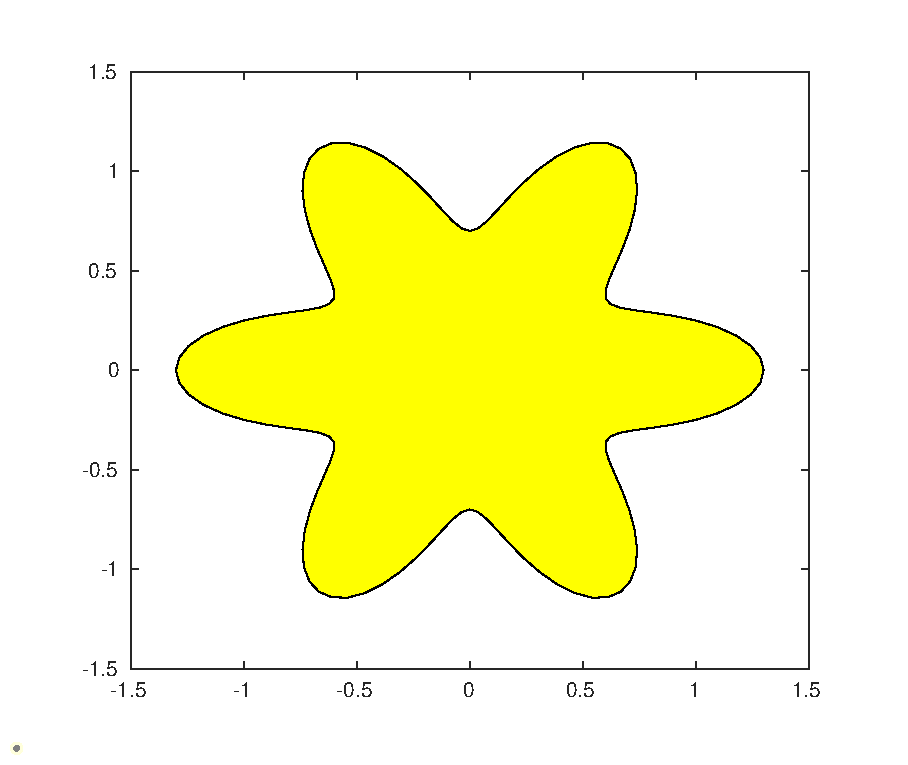
\includegraphics[width=0.3\linewidth]{star_originfill.eps}
    }
	\subfigure{
		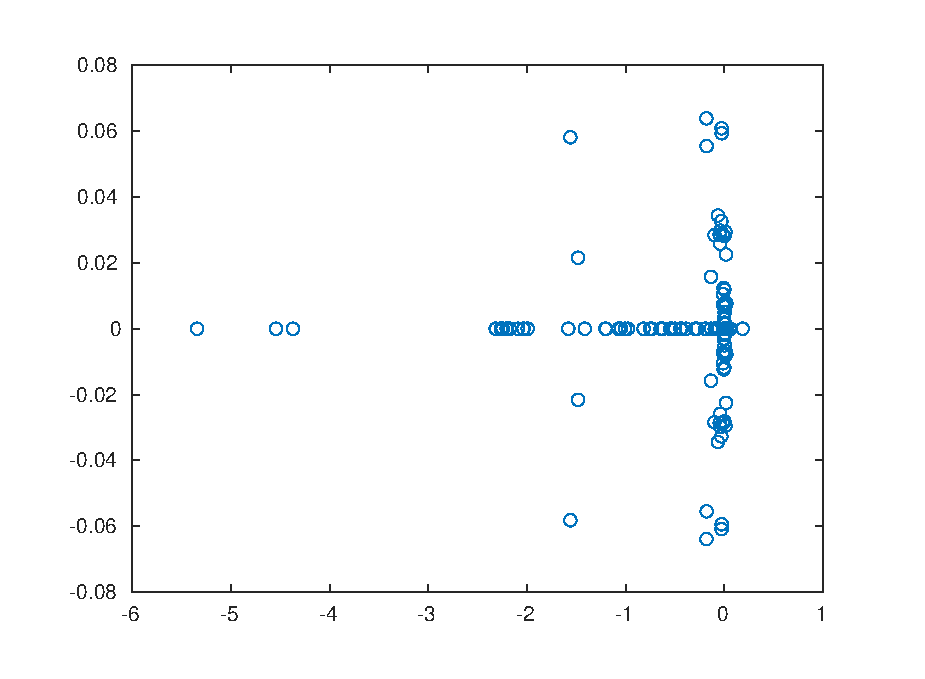
\includegraphics[width=0.3\linewidth]{Eigenvalues_0.eps}
    }\\
    \subfigure[$t=0.0005$]{
        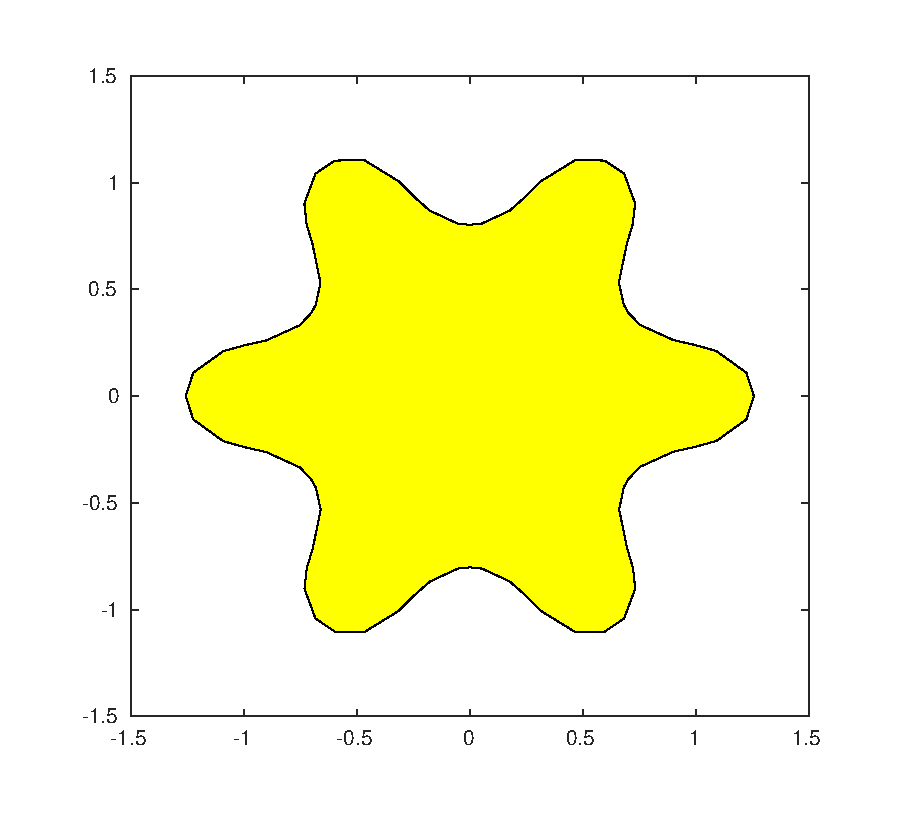
\includegraphics[width=0.3\linewidth]{star_ESDIRK64_0.0005.eps}
      }
      \subfigure{
        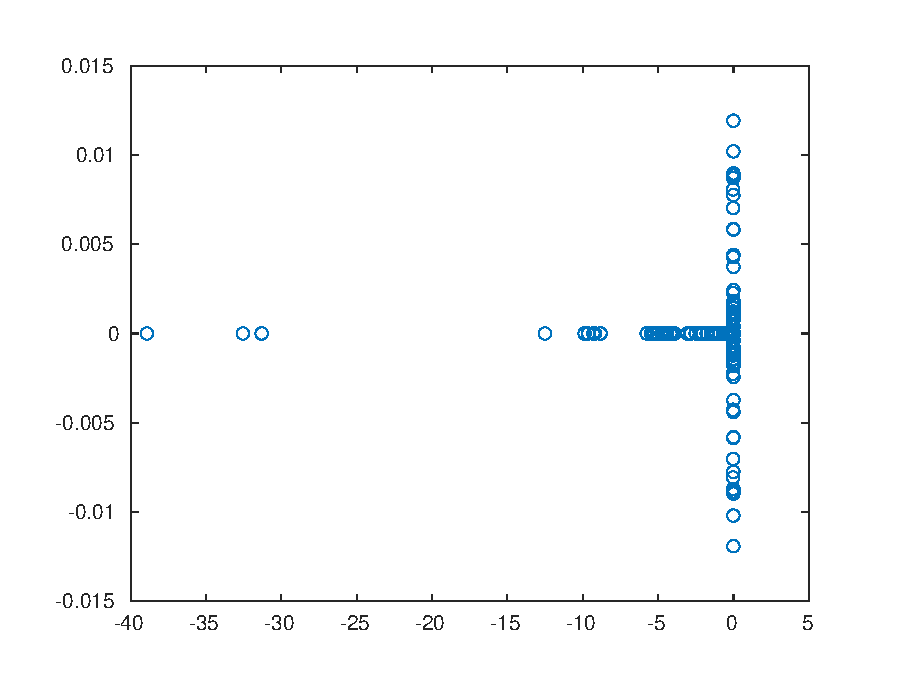
\includegraphics[width=0.3\linewidth]{Eigenvalues_0.0005.eps}
    }\\
    \subfigure[$t=0.002$]{
		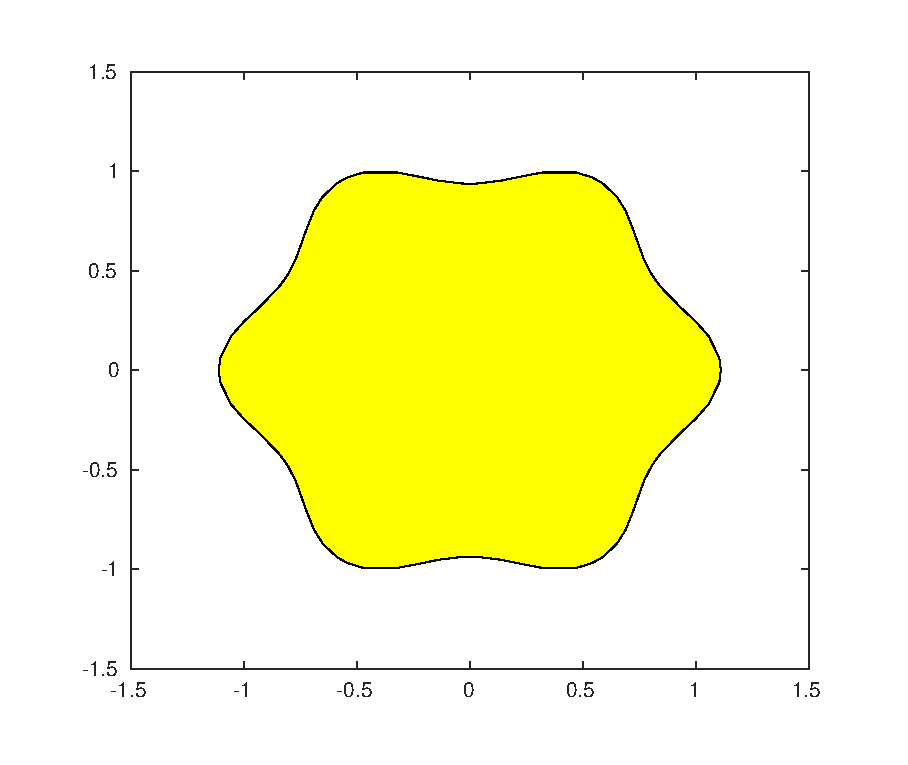
\includegraphics[width=0.3\linewidth]{star_ESDIRK64_0.002.eps}
    }
	\subfigure{
		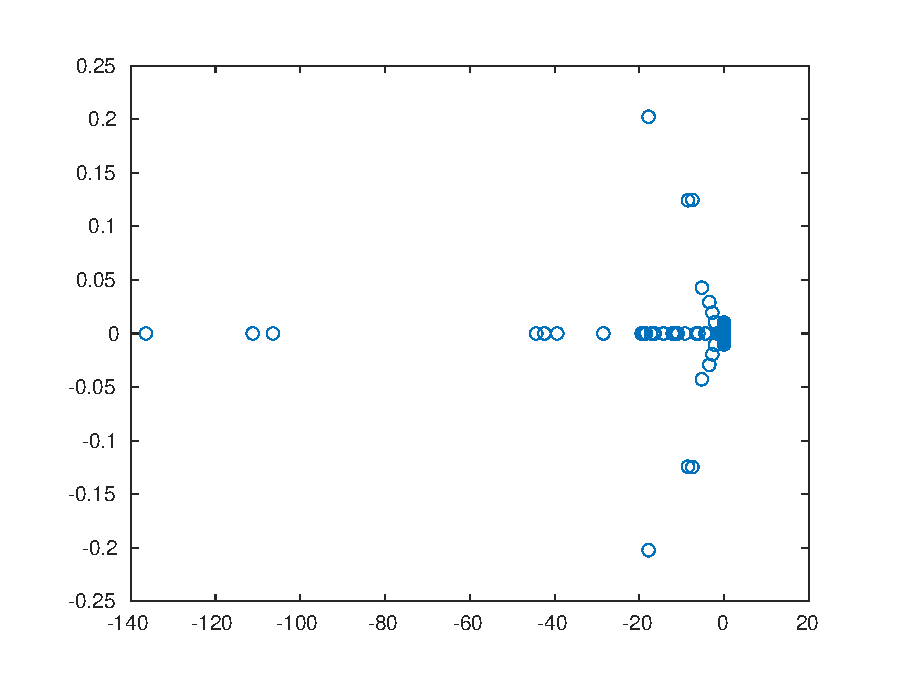
\includegraphics[width=0.3\linewidth]{Eigenvalues_0.002.eps}
    }\\
    \subfigure[$t=0.006$]{
        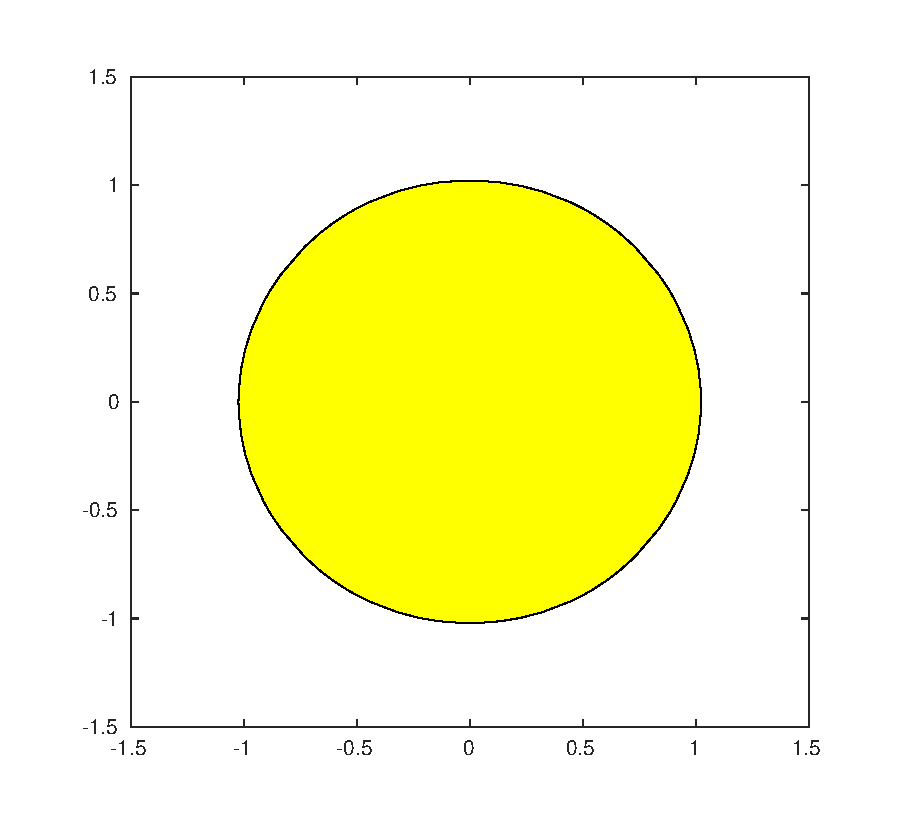
\includegraphics[width=0.3\linewidth]{star_ESDIRK64_0.006.eps}
      }
      \subfigure{
        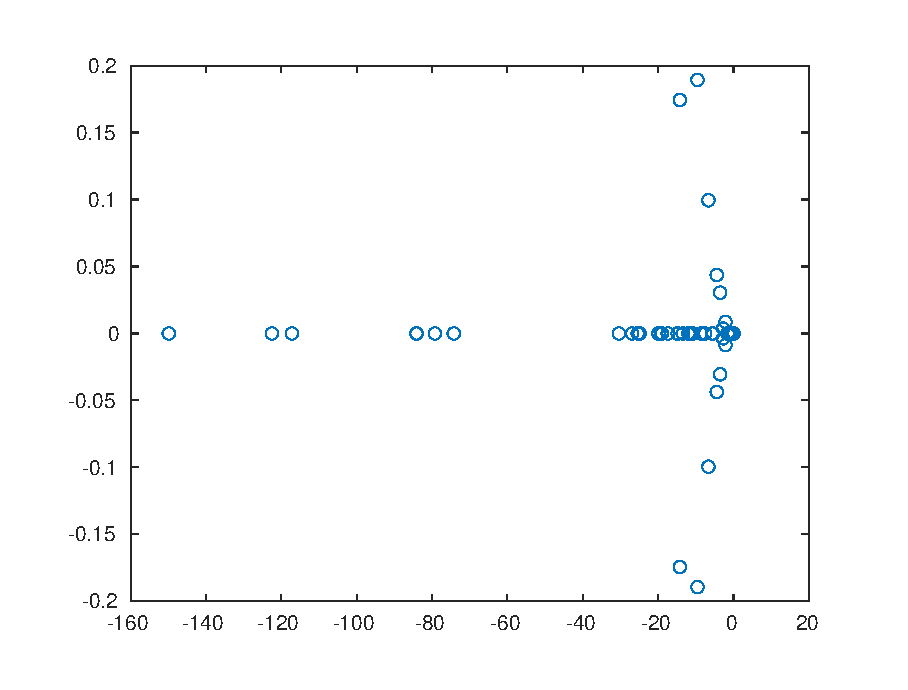
\includegraphics[width=0.3\linewidth]{Eigenvalues_0.006.eps}
    }
    \caption{四阶方法曲线和雅可比矩阵$J_{\boldsymbol f_{\bar{s}}}$特征
      值乘$1/n^2$后的分布,$n=64$,$k=$ 5e-7,$r_\mathrm{tiny}=0.01$,
      结束时间$t_e = 0.6$。}
    \label{fig:Eigenvlaues}
  \end{figure}
  从上图可以看出,雅可比矩阵的特征值的分布基本沿虚轴和负实轴。在初始时
  刻点分布较均匀的情况下,谱半径较小,随着时间推移,后续步骤中谱半径约
  为初始值的20倍。对二阶方法的分析可以得到相似的结果。
\newpage
\begin{thebibliography}{99}  
\bibitem{ref1}C. M. Elliott and H. Garcke, Existence results for geometric interface models for surface
diffusion, Adv. Math. Sci. Appl., 7 (1997), pp. 467–490.
\bibitem{ref2}A. Polden, Curves and surfaces of least total curvature and forth-order flows, Ph.D. dis-
sertation, Universität Tübingen, Germany (1996).
\bibitem{ref3}Y. Giga and K. Ito, On pinching of curves moved by surface diffusion, Comm. Appl. Anal.,
2 (1998), pp. 393–405
\bibitem{ref4}J. Escher, U.F. Mayer, G. Simonett, The surface diffusion flow for immersed hypersurfaces, SIAM J. Math. Anal. 29 (1998) 1419–1433.
\bibitem{ref5}Y. Giga and K. Ito, Loss of convexity of simple closed
  curves moved by surface diffusion. topics in nonlinear analysis the
  herbert amann anniversary volume.(1998)
\bibitem{ref6}Qinghai Zhang, Fourth- and Higher-order Interface Tracking via Mapping and Adjusting Regular Semianalytic sets Represented by Cubic Splines, SIAM Journal on Scientific Computing, 40(6), 2018.
\bibitem{ref7}Qinghai Zhang and Aaron Fogelson, MARS: An analytic framework of interface tracking via mapping and adjusting regular semialgebraic sets, SIAM Journal on Numerical Analysis, 54(2), 2016.

\end{thebibliography}
\end{document}

